\documentclass[a4paper,oneside]{book} 
% the 'oneside' option makes viewing on a computer easier, as both inner and outer margins are equal. Change this while printing.

\usepackage{amsmath,amssymb}
\usepackage{hyperref}
\usepackage{amscd}
\usepackage{amsthm}
\usepackage{color}

\usepackage[T1]{fontenc}

\usepackage{enumerate} % Customize the enumerate environment
\usepackage{mathtools} % for \prescript

%\usepackage{cite}
\usepackage{bm} 

\usepackage[vcentermath]{youngtab} % Excellent package for young diagrams

% For compact lists. Provides the environments 
%   itemize*, enumerate*, description*
% with lesser spacing between items.
\usepackage{mdwlist} 
\usepackage{enumerate} 

\usepackage{mathtools} % For 'Aboxed' command

% Theorem-like environments
\usepackage{amsthm}
\theoremstyle{definition}
\newtheorem{definition}{Definition}

\theoremstyle{plain}
\newtheorem{theorem}{Theorem}
\newtheorem{corollary}{Corollary}
\newtheorem{conjecture}{Conjecture}
\newtheorem{lemma}{Lemma}
\newtheorem{proposition}{Proposition}

% TikZ
\usepackage{tikz}
\usepackage{tikz-cd} % Commutative Diagrams in TikZ
\usetikzlibrary{positioning}
\usetikzlibrary{decorations.pathreplacing} % for curly braces
\usetikzlibrary{decorations.pathmorphing} % for squiggly arrows
\usetikzlibrary{calc} % for coordinate calculation
% Tikz Style for Commutative Diagrams
\tikzset{
    commutative diagram/.style={
            node distance=2cm,auto,
            arrow/.style={-stealth},
            exists/.style={-stealth,densely dotted}
        }
    }

% This compactifies a list by removing unnecessary whitespace
\newcommand\makethislistcompact{
        \setlength{\itemsep}{0pt}%
        \setlength{\parskip}{0pt}%
        %\setlength{\topsep}{50pt} 
        %\setlength{\partopsep}{10pt}
        %\setlength{\parsep}{50pt}
}
% Framed environments
\usepackage[framemethod=tikz]{mdframed}

% Common operators
\DeclareMathOperator\GL{GL}  % General Linear Group
\DeclareMathOperator{\Image}{Im} % Image
\DeclareMathOperator{\Coker}{Coker} % Cokernel 
\DeclareMathOperator{\Ker}{Ker} % Kernel
\DeclareMathOperator{\Tr}{Tr} % Trace
\DeclareMathOperator{\Hom}{Hom} % Homomorphisms
\DeclareMathOperator{\End}{End} % Endomorphisms
\DeclareMathOperator{\Aut}{Aut} % Automorphisms
% Commonly used sets
\newcommand{\CC}{\mathbb{C}}
\newcommand{\RR}{\mathbb{R}}
\newcommand{\ZZ}{\mathbb{Z}}
\newcommand{\HH}{\mathbb{H}}
\newcommand{\FF}{\mathbb{F}}
\newcommand{\uhp}{\mathcal{H}}
\newcommand{\SL}{\text{SL}}

\renewcommand{\>}{\rangle}
\newcommand{\<}{\langle}

% Some semantically named symbols
\newcommand\isomorphic\cong

% Meta-notes
\newcommand\Solution[2]{\emph{[Solution to Exercise #1 in #2]}}
\newcommand\Todo[1]{\begin{color}{red}{#1}\end{color}}
\newcommand{\tocheck}[1]{{\color{red} #1}}
\newcommand{\comment}[1]{{\color{cyan} #1}}

% Environment for "physical insights"
\newenvironment{insight}
  {\begin{mdframed}[%style=2,%
      leftline=true,
      rightline=true,
      topline=false,
      bottomline=false,
      leftmargin=2em,
      rightmargin=2em,%
      innerleftmargin=1em,
      innerrightmargin=1em,
      linewidth=2pt,%
      linecolor=white!70!black,%
      %backgroundcolor=white!99!black, %
      skipabove=7pt,skipbelow=7pt]\small}
  {\end{mdframed}}

%%%%%%%%%%%%%%%%%%%%%%%%%%%%%%%%



% Bibliography
\usepackage[
    backend=bibtex,
    %style=authoryear-icomp,
    style=alphabetic,
    sortlocale=de_DE,
    natbib=true,
    url=false, 
    doi=true,
    eprint=false
]{biblatex}
\addbibresource{repth.bib}


\usepackage[vcentermath]{youngtab} % Excellent package for young diagrams
\setcounter{secnumdepth}{1}

% Some common representations
\DeclareMathOperator{\Sym}{Sym} % Symmetric product
\DeclareMathOperator{\Alt}{\Lambda} % Exterior product
\DeclareMathOperator{\sgn}{sgn} % Alternating representation
\DeclareMathOperator{\triv}{triv} % Trivial representation
\DeclareMathOperator{\std}{std} % Standard representation
\DeclareMathOperator{\Ind}{Ind} % Induced representation 

% Some common maps
\DeclareMathOperator{\id}{id}

\DeclareMathOperator{\gr}{gr}

% Semantic stuff
\newcommand{\onto}{\twoheadrightarrow}
\newcommand{\Lie}[1]{\mathfrak{#1}}

% Some common lie algebras
\newcommand{\LieGL}{\mathfrak{gl}}
\newcommand{\LieA}{\mathfrak{a}}
\newcommand{\LieB}{\mathfrak{b}}
\newcommand{\LieG}{\mathfrak{g}}
\newcommand{\LieH}{\mathfrak{h}}
%\newcommand{\sl}{\mathfrak{sl}}

% Some common lie algebra ideals
\DeclareMathOperator\Rad{Rad}


%%%%%%%%%%%%%%%%%%%%%%%%%%%%%%%%

% Title
\title{Representation Theory}
\author{Hersh Singh}
\begin{document}
\maketitle

\tableofcontents

\chapter{Representations of Finite Groups}
\section{Definitions}
\label{sec:definitions}

Let $G$ be a finite group, $V$ be a finite dimensional complex vector space.

A \emph{representation} of $G$ on $V$ is a group homomorphism 
\begin{align}
    \rho:  G\to \GL(V), 
\end{align}
where $\GL(V)$ is the group of automorphisms of $V$. Even though the ``representation" is really the the vector space $V$ \emph{and} the homomorphism $\rho$, but it is common (especially by physicists) to refer to $V$ itself as the representation. 

\begin{insight}
We say that this map gives $V$ the structure of a G-module. This agrees with the  definition of a R-module (R is a ring) that I have studied earlier. An R-module is simply a vector space defined over a ring, instead of a field. So the ring elements act as the \emph{scalars}. Of course, the description must include a rule for the `interaction' of the scalars with the vectors. To be a module, the interaction must be \emph{linear}.  
In this case, the group homomorphism $\rho$ gives us that rule of interaction between the vectors (elements of $V$) and the scalars (elements of $G$). For $g\in G, v \in V$, $$gv\equiv\rho(g)v \in V$$
\end{insight}


A vector space homomorphism $\phi: V\to W$ is a morphism between the two representations $V$ and $W$ if the following diagram commutes:
\begin{equation} \begin{CD}
  V @>\phi>> W\\
  @VgVV @VVgV\\
  V @>\phi>> W\\
\end{CD} \end{equation}

That is, $\phi g=g\phi$ for all $g\in G$. This makes the group elements \emph{behave like scalars under module homomorphisms}. Such morphisms of representations are also called $G$-\emph{linear map} or a \emph{$G$ intertwiner}.

\begin{insight}
   Why is this is a good definition? Seems to be inspired from module homomorphisms. This is natural in some sense - Figure that out.
\end{insight}

$\Ker \phi,\ \Image \phi,\ \Coker \phi = V/\Image\phi$ are also $G$-modules. This is solely because of the commutativity of the above diagram.
\begin{itemize}
    \item If $v\in \Ker \phi$, then $\phi(gv) = g\phi(v) = 0$. So $gv$ also $\in \Ker \phi$. $\blacksquare$.
    \item If $v\in \Image \phi$, then let $\phi(v) = w$. So $\phi(gv)=g\phi(v)=gw \in W$. So $gv$ also $\in \Image \phi$. $\blacksquare$.
\end{itemize}

One of the goals of our study is, given a representation, to develop tools for constructing other, preferably all, representations of the group. 
Some examples of representations that can be constructed from $V$ and $W$

\begin{enumerate}[(a)]
    \item Tensor product $V\otimes W$ via
        \begin{align}
            g(v\otimes w) = g(v) \otimes g(w)
        \end{align}
    \item Tensor power $V^{\otimes n}$ and the \emph{exterior power}  $\Lambda^n(V)$ and the \emph{symmetric power} $\Sym^n(V)$ are its subrepresentations.
    \item the dual $V^* = \Hom(V,\CC)$. This is a little tricky though. The action of $G$ on $V^*$ must be such that it preserves the natural inner product, denoted by $\<\ ,\ \>$, between them. So, if we have a representation $(V^*,\rho^*)$ and $(V,\rho)$, then we should have
        \begin{align}
            \rho^*_g(u^*)(\rho_g v) = u^*(v)
        \end{align}
        where I have written $\rho_g=\rho(g)$ for a cleaner notation, and $u^*\in V^*,\ v\in V$. 
        \begin{insight}
            Remember the definition of the transpose map. If we have a map $f: V\to W$, then the transpose of $\rho$ is a map $^t\rho: W^*\to V^*$ such that
            \begin{align}
                ^tf(\phi) = f\cdot \phi \quad\quad\forall \phi\in W^*.
            \end{align}
            It's a good idea to make commutative diagrams out of statements like the above:
            \begin{center}
            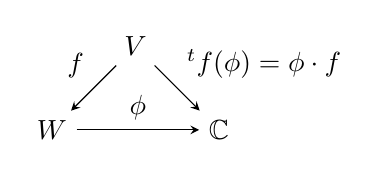
\begin{tikzpicture}[commutative diagram, node distance=1.5cm]
                \node (V) {$V$};
                \node (CC) [below right of=V] {$\CC$};
                \node (W) [below left of=V] {$W$};
                \draw [arrow] (V) -- (CC) node [midway] {$^tf(\phi)=\phi\cdot f$};
                \draw [arrow] (V) -- (W) node [midway,auto=right] {$f$};
                \draw [arrow] (W) -- (CC) node [midway] {$\phi$};
            \end{tikzpicture}
            \end{center}
        \end{insight}
        If we now define
        \begin{align}
            \rho^*(g) &= \prescript{t}{}\rho(g^{-1})
            \label{eqn:defn_dualrep}
        \end{align}
        we get
        \begin{align*}
            \rho_g^*(u*)(\rho_g v) &= \prescript{t}{}\rho_{g^{-1}}(u^*)(\rho_g v)\\
                &= u^*\cdot\rho_{g^{-1}} (\rho_g v) \\
                &= u^* (\rho_{g^{-1}g} v) \\
                &= u^*(v).
        \end{align*}
        The definition \eqref{eqn:defn_dualrep} preserves the inner product, and is a thus a sane definition.
    \item $\Hom(V,W)$ by the identification, $\Hom(V,W)=V^*\otimes W$ (see appendix \ref{cha:tensor_product}). If $(\phi: V\to W)\in \Hom(V,W)$ then let $\sum_i \phi_{ij} v_i^*\otimes w_j$. Writing out the action of this on $u\in V$,
        \begin{align*}
            (g\phi)(gu) &= \left[ g \sum\phi_{ij} v^*_i \otimes w_j \right] (gu) \\
                &= \Big[ \sum_{ij}\phi_{ij} gv^*_i \otimes gw_j \Big] (gu) \\
                &= \sum \phi_{ij} \<gv_i^*, gu\> g w_j\\
                &= \sum \phi_{ij} \<v_i^*, u\> g w_j\\
        \end{align*}
        This gives us
        \begin{align}
            (g\phi)(gu) &= g\cdot\phi(u)\quad \forall u\in  V.
            \label{eqn:linearmap_groupaction}
        \end{align}
        \begin{insight}
            Note that you cannot multiply both sides by $g^{-1}$ to imply that $\phi(gu)=\phi(u)$. This can't be done since the action of $G$ on $V^*$ is \emph{not associative}. That means,
            \begin{align*}
                (g\phi)(u) \neq g\cdot \phi(u),
            \end{align*}
            as can be seen by simply taking, say, $\phi=v^*\otimes w$. LHS becomes $\< gv^*, u \>gw$ while RHS becomes $\<v^*,w\>gw$.
        \end{insight}
        \begin{center}
            \begin{tikzpicture}[commutative diagram]
                \node (V1) {$V$};
                \node (W1) [right of=V] {$W$};
                \node (V2) [below of=V1] {$V$};
                \node (W2) [below of=W1] {$W$};
                \draw [arrow] (V1) -- (W1) node [midway, auto=right] {$\phi$};
                \draw [arrow] (V2) -- (W2) node [midway, auto=right] {$g\phi$};
                \draw [arrow] (V1) -- (V2) node [midway, left] {$g$};
                \draw [arrow] (W1) -- (W2) node [midway] {$g$};
            \end{tikzpicture}
        \end{center}
        Ofcouse, if $\phi$ is a $G$-linear map (a map between reprentations $V$ and $W$), then we also have $g\cdot\phi = \phi\cdot g$ for all $g\in G$. Consider the space $\Hom_G(V,W) \subset \Hom(V,W)$, which consists of maps from $V$ to $W$ invariant under the action $G$. If $\phi\in \Hom_G(V,W)$, then we have $(g\phi)(gu)=g\phi(u)$ and $(g\phi)(u)=\phi(u)$ (by invariance of the map under $G$). Thus we have $g\phi(u)=\phi(gu)$. The converse is also easily seen to be true.Therefore, $\Hom(V,W)$ is space of all $G$-linear maps $V\to W$.  \Solution{1.2}{FH} 

        
\end{enumerate}



\begin{itemize}
    \item \Todo{Todo: Regular Representation}
    \item \Todo{Exercise 1.3,1.4}
\end{itemize}

\section{Schur's Lemma}
\label{sec:schur_s_lemma}

\begin{lemma}[Schur's Lemma]
    Let $V,\ W$ be irreps of a group $G$ and $\phi: V\to W$ a $G$-linear map. Then,
    \begin{enumerate}[(i)]
        \item either $\phi$ is 0 or an isomorphism;
        \item if $V=W$, then $\phi=\lambda I$.
    \end{enumerate}
\end{lemma}

\section{Examples}
\label{sec:examples}

We observe that any $g\in G$ gives a map $\rho(g): V\to V$. In general, this is not a $G$-linear map however. For $\rho(g)$ to be a $G$ linear map, ...
%\begin{align}
    %g(h(v)) &= h(g(v))\quad\quad \forall h\in G
%\end{align}
%which just says that the set of all $G$-linear maps in $\rho(G)$ is precisely the center of $G$, given by $Z(G)$.

\subsection{Abelian Groups}
\label{sub:abelian_groups}

If $G$ is an abelian group, and $V$ is an irrep, then $\rho(g)$ is a $G$-linear map.By Schur's Lemma, $\rho(g)=\lambda I$. That means that any proper subspace of $V$ is actually invariant under the action of $G$, and is a thus a subrepresentation. But since $V$ is irreducible, this can only mean that $V$ has no non-trivial proper subspace, which implies that $V$ is one-dimensional. Therefore, any representation of an abelian group is just an element of the \emph{dual group}
\begin{align}
    \rho: G \to \CC^*.
\end{align}

%Incidentally, this is also the definition of the \emph{dual group}.

\subsection{\texorpdfstring{$S_3$}{S3}}
%\label{sub:_s_3_}

\begin{insight}
    Remember that $S_3$ is the group of permutations of three objects. Algebraically, it can be thought to be generated by the elements
    \begin{align}
        \{1,\ \tau,\ \tau^2, \sigma,\ \sigma\tau,\ \sigma\tau^2\}
    \end{align}
    subject to the conditions
    \begin{align}
        \tau^3=1,\quad \sigma^2=1,\quad (\sigma\tau)^2=1.
    \end{align}
    You can tell that $\sigma$ is a 2-cycle and $\tau$ is a 3-cycle.
    
\end{insight}

Lets now discuss the case of the \emph{simplest non-abelian group}, $S_3$. We already know three representations to begin with:
\begin{enumerate}[(i)] 
    \makethislistcompact
    \item the trivial representation,
        \begin{align}
            \rho(g) &= I
        \end{align}
    \item the alternating representation
        \begin{align}
            \rho(g) &= \sgn(g),
        \end{align}
    \item the natural permutation representation.\\
        But this is not irreducible. It can be easily seen that the subspace spanned by the vector $(1,1,1)$ is invariant under $G$. So, the space $V$ complimentary to it is another (hopefully irreducible!) representation. If $v=(z_1,z_2,z_3) \in V$, then 
        \begin{align}
            (z_1,z_2,z_2)\cdot(1,1,1) &= 0\\
            \implies z_1 + z_2 + z_3 &= 0.
        \end{align}
        We thus have
        \begin{align}
            V &= \{(z_1,z_2,z_3) \in \CC^3: z_1 + z_2 + z_3 =0\}.
        \end{align}
        Now if this further has an invariant subspace, it must be spanned by an element of the form $(z_1,z_2,-z_1-z_2)$. Applying a few permutations will convince you immediately that this is not an invariant subspace. Therefore, the representation we have is irreducible, called the \emph{standard representation} of $S_3$.
\end{enumerate}
We now want to characterize any arbitrary representation $W$ of $S_3$. To do so, we first look at the action of the abelian subgroup $ U_3 = \ZZ/3 \in G$ (generated by $x$) on $W$. If $v\in W$ is an eigenvector of $\rho(x)$, then 
\begin{align}
    \tau \sigma (v) &= \sigma\tau^2 (v)\\
        &= \omega^2 (\sigma v)
\end{align}
This means that if $v$ is eigenvector of $\tau$ with the eigenvalue $\omega$, then $\sigma v$ is also an eigenvector with the eigenvalue $\omega^2$.
To find the decomposition of the $W$, we go through the following steps:
\begin{enumerate}[(i)]
    \item Start with an eigenvector $v$ of $\tau$, which has the eigenvalue $w^i$.
    \item If $w^i\neq 1$, then $\sigma v$ is an eigenvector independent of $\tau$ with the eigenvalue $w^{2i}$. In this case, $\{v,\sigma v\}$ form a two dimensional subspace of $W$ invariant under $S_3$ (as $\sigma$ just exhanges $v$ and $\sigma v$). In fact, this subrepresentation is isomorphic to the standard representation and is thus irreducible.
    \item If $w^i = 1$, then $\sigma v$ may or may not be independent of $v$.
        \begin{enumerate}
            \item If $\sigma v$ is independent of $v$, then $v + \sigma v$ spans a subspace isomorphic to the trivial represntation and $v - \sigma v$ spans a subspace isomorphic to the alternating representation. 
            \item If $\sigma v$ and $v$ are not linearly independent, then 
                $\sigma v= \lambda v$ for some $\lambda\in \{1,-1\}$ (since $\sigma^2=I$). If $\lambda=1$, then $\CC v$ is isomorphic to the trivial representation and if $\lambda=-1$, then $\CC v$ is isomorphic to the alternating representation.
        \end{enumerate}
\end{enumerate}

Note that this allows to find all irreps of a given representation $W$!

\Solution{1.12(a)}{FH} Lets use this approach to find out the irreps of th regular representation $R$ of $S_3$. A general vector in the space looks like this
\begin{align}
    v &= a_1 + a_2 \tau + a_3 \tau^2 + b_1\sigma + b_2 \sigma\tau + b_3\sigma \tau^2 
\end{align}

The eigenvalues of $\tau$ are $\{1,\omega,\omega^2\}$. 
\begin{enumerate}
    \makethislistcompact
    \item For eigenvalue $=1$, we have $v=1 + \tau + \tau^2$ and $\sigma v = \sigma + \sigma\tau + \sigma\tau^2$. Thus $\CC (v+\sigma v)\isomorphic \triv$ and $\CC (v-\sigma v) \isomorphic \sgn$ are two irreps.
    \item For eigenvalue $=\omega$, we get on solving $\tau \alpha = \omega \alpha$
        \begin{align}
            \alpha &= \omega^2\tau + \omega\tau + \tau^2
        \end{align}
        With $\beta = \sigma \alpha$, we get the subspace spanned by $\{\alpha,\beta\}$ to be isomorphic to the standard representation.
    \item For eigenvalue $=\omega^2$, we get 
        \begin{align}
            \alpha' &= \omega^2 + \omega\tau + \tau^2\\
            \beta' = \sigma\alpha &= \omega^2\sigma + \omega\sigma\tau + \sigma\tau^2
        \end{align}
        The subspace spanned by $\{\alpha',\beta'\}$ is again isomorphic to the standard representation.
\end{enumerate}
We have enumerated six linearly independent eigenvectors and therefore exhausted all of them. We thus get
\begin{align}
   R &\isomorphic \triv \oplus \sgn \oplus (\std)^2 \quad\quad\square    
\end{align}
\Solution{1.14}{FH} For an irrep $V$ of a finite group $G$, there is a unique Hermitian inner product preserved by $G$. Say there are two Hermitian products, $H$ and $H'$, preserved by $G$. Any Hermitian inner product sets up an isomorphism between $V$ and $V^*$. Let that map be given by
\begin{align}
    \phi_1(v) &= H_1(v,\cdot) \in V^*\\
    \phi_2(v) &= H_2(v,\cdot) \in V^*
\end{align}
\begin{insight}
    Write details about the isomorphism between $V$ and $V^*$. Crucial is the positive-definiteness of the inner product. Not sure where the Hermiticity of the inner product is important.
\end{insight}
\begin{align}
    V^* \xleftarrow{\phi_1} V \xrightarrow{\phi_2} V^*
\end{align}
Now, the map $\phi = \phi_2\cdot\phi_1^{-1}$ is an isomorphism of vector spaces. It is also a $G$-linear map since its the composition of $G$-linear maps. Therefore, $\phi$ is an isomorphism between two irreps. By Schur's lemma, $\phi=\lambda\cdot I$, where $\lambda$ is any scalar. This gives us
\begin{align}
    H_2(v,\cdot) &= \phi(H_1(v,\cdot)) \\
        &= \lambda H_1(v,\cdot)\quad\quad\qed
\end{align}

\noindent\Todo{\Solution{1.13(a)}{FH}}\\
\Solution{1.13(b)}{FH} Is $\Sym^n(\Sym^mV)\isomorphic \Sym^m(\Sym^n V)$? No, since the dimensions don't match on both sides.
\begin{align}
    \dim \Sym^n(\Sym^mV) &= ^{{}^{\dim V - 1 + m}C_{m} -1 +n}C_{n}
\end{align}
The above equation is clearly not symmetric in $m$ and $n$. So the isomorphism can not hold in general.


\chapter{Character Theory}
\label{cha:character_theory}
\begin{definition}
    If $V$ is a representatin of $G$, its \emph{character} $\chi_V$ is the complex-valued functin on the group defined by
    \begin{align}
        \chi_V(g) &= \Tr(g|_V),
    \end{align}
    the trace of $g$ on $V$.
\end{definition}

We shall drop the subscript $V$ when it's obvious.

Some properties
\begin{enumerate}
    \item $\chi_V$ is a class function, which means that it is constant on conjugacy classes  of $G$.
        \begin{align}
            \chi(hgh^{-1}) &= \chi(g)
        \end{align}
    \item 
\end{enumerate}

\section{First Projection Formula}
\label{sec:first_projection_formula}
Let us define $V^G$ as the elements of $V$ fixed under the action of $G$.
\begin{align}
    V^G=\{v\in V: gv=v\ \forall g\in G \}
\end{align}
The sub space $V^G$ is actually the direct sum of the trivial subrepresentations.

Now, the endomorpism $\varphi \in \End(V)$, 
\begin{align}
    \varphi &= \frac{1}{|G|} \sum_{g\in G} g
\end{align}
is $G$ linear, since $h\varphi h^{-1} = \frac{1}{|G|}\sum_{g\in G} hgh^{-1} = \varphi$.  Infact, $\varphi$ is projection of $V$ to $V^G$.

So, now we have a way of finding the direct sum of the trivial subreprentations of $V$. The trace of this map is would be the dimension of $V_G$ [\Todo {Why?}], which is the number of copies of trivial representations in $V^G$.

\begin{insight}
    \Todo{ For an arbitrary linear map (projection?) $T: V\to W$, do we have $\Tr T =\dim W$ ?  }
\end{insight}

\begin{align}
    \dim V^G &= \Tr (\varphi)\\
        &= \frac{1}{|G|}\sum_{g\in G} \Tr(g)\\
        &= \frac{1}{|G|}\sum_{g\in G}\chi_V(g)
        \label{eqn:dimV_G}
\end{align}
In particular, if $V$ is irreducible, then it has no trivial subrepresentations and thus
\begin{align}
    \sum_{g\in G} \chi_V(g) &= 0\quad\quad\text{if $V$ is an nontrivial irrep}.
\end{align}

We know that $\Hom(V,W)^G$, the set of all homorphisms $V\to W$ fixed under $G$, is just the space of all $G$-linear maps $V\to W$. [\Todo{reference here.}]
\begin{insight}
    Given a $G$-linear map $\phi: V\to W$, where $V$ is a an irrep, $\phi$ defines an isomorphism between $V$ and $\Image(\phi)$ (since $\ker \phi$ is a subrepresentation of $V$, and so must be $\{0\}$) Now, other such $\phi$ would give us copies of $V$ in $W$. \Todo{The dimensionality of the space $\Hom_G(V,W)$ thus tells us the multiplicity of $V$ in $W$.}
\end{insight}

By Schur's lemma, if $V$ and $W$ are both irreducible then
\begin{equation}
    \dim \Hom_G(V,W) = 
        \begin{cases}    
            1   &\text{if } V\isomorphic W \\
            0   &\text{if } V\ncong  W
        \end{cases}
\end{equation}
Since we have $\Hom_G(V,W)\isomorphic V^*\otimes W$,
\begin{align}
    \chi_{\Hom_G(V,W)}(g) &= \overline{\chi_V(g)}\cdot\chi_W(g)
\end{align}
Using \eqref{eqn:dimV_G} here, we get the nice result
\begin{align}
        %\frac{1}{|G|}\sum_{g\in G}\chi_V(g) &= 
        \frac{1}{|G|}\sum_{g\in G} \overline{\chi_V(g)}\cdot\chi_W(g) 
        &= \begin{cases}    
            1   &\text{if } V\isomorphic W \\
            0   &\text{if } V\ncong  W
        \end{cases}
\end{align}
This inspires us to define a dot product on the space of all class functions (functions that are defined on the conjugacy classes of a group) of $G$,
\begin{align}
    \CC_{\text{class}}(G) &= \{\text{class functions on $G$}\},
\end{align}
as
\begin{align}
    (\alpha,\beta) &= \frac{1}{|G|} \sum_{g\in G} \overline{\alpha(g)} \beta(g).
    \label{eqn:dotproduct_classfunctions}
\end{align}
In respect this dot product, the characters of irreps are orthornormal.

\chapter{Induced Reprentations}
\label{cha:induced_reprentations}

\section{Overview}
%\label{sec:overview}
\begin{enumerate}
    \makethislistcompact
    \item Define induced representations
    \item Mackay formula for the character of an induced representation.
    \item Frobenius Reciprocity
\end{enumerate}

\section{Definitions}

\Todo{Don't really understand the motivation for this section.}
\emph{Reference: Etingof.}

Given a subgroup $H\subset G$, and $(\rho_V, V)$, a representation of $G$, we can easily construct a representation for $H$ by simply restricting $\rho_V$ to $H$, which we denote by $\rho_V|_H$.

However, if want to construct a representation of $G$ from a representation of $H$, then we need to think a little more about it. 

Think of the elements of $V$ as functions of $G$, that is, every element $v\in V$ defines a map $v: G\to V$ given by
\begin{align}
    v(g) &= \rho(g) v.
\end{align}
Now, we already know how $v(\cdot)$ acts on $H$. We want to extend that action to $G$. The least we could do is to ensure that the action on $G$ is consistent with the known action on $H$. So, we enforce that
\begin{align}
    v(hg) = h\cdot v(g) &= \rho_V(h) v(g)\quad \forall h\in H,\ g\in G.
\end{align}

\begin{insight}\Todo{
    Why is $\Ind_H^G{V}$ naturally isomorphic to $\Hom_H(k[G],V)$?
    }
\end{insight}

\chapter{Representations of \texorpdfstring{$S_n$}{Sn}}
\label{cha:representations_of_s_n}



\section{Overview}

\begin{enumerate}
    \makethislistcompact
    \item Represenations of $S_n$
    \item Frobenius Formula for the character/dimension of a representation of $S_n$
    \item Schur Functors
\end{enumerate}

\section{Representations}
%\label{sec:representations}


\begin{enumerate}
    \makethislistcompact
    \item Define the standard Young tableau, given by a partition $\lambda$.
    \item Define the subgroups $A_\lambda,\, B_\lambda$ of $S_n$ that act only on rows and columns of the tableau, respectively.
    \item Define the \textbf{Young symmtrizer},
        \begin{align}
            c_\lambda = \sum_{\substack{\alpha\in A,\, \beta\in B}} \alpha \beta \sgn(\beta).
        \end{align}
    \item For some $x\in G$, if $\alpha x \sgn(\beta)\beta = x$ for all $\alpha\in A,\, \beta\in B$, then $x$ is a scalar multiple of $c_\lambda$.
    \item The set $\{(\CC S_n )c_\lambda : \lambda \text{ is a partition of } S_n\}$, with $S_n$ acting on the left by multiplication, is the set of all representations of $S_n$.
\end{enumerate}


\chapter{A Detour to Differential Geometry}
\label{cha:a_small_detour_to_differential_geometry}

\begin{enumerate}
    \makethislistcompact
    \item Manifolds
    \item Morphism of manifolds -  Smooth mappings etc
    \item Types of submanifolds - Immersion, Embedding etc
    \item Tangent Spaces
    \item Differential forms
\end{enumerate}




\chapter{Lie Groups}
\label{cha:lie_groups}

\section{Overview}
\label{sec:overview}

\begin{enumerate}
    \makethislistcompact
    \item Define Lie groups
    \item Two principles
    \item Vector fields, differential forms
    \item The Lie bracket: two ways to define it.
    \item The transition: Lie groups $\to$  Lie algebras
    \item Adjoint representation
    \item Examples of Lie algebras - from classical groups
    \item Exponential map
    \item Apply the exponential map to Lie groups
\end{enumerate}




\chapter{Campbell-Baker-Hausdorff}
\section{}
We describe the algebraic proof of the CBH formula. 

\begin{enumerate}
    \makethislistcompact
    \item Define universal enveloping algebra
    \item Define the tensor algebra
    \item Show that universal enveloping algebra and the tensor algebra are canonically isomorphic
    \item Poincare-Birkhoff-Witt theorem
\end{enumerate}

\subsection{Universal enveloping algebra}
\label{sub:universal_enveloping_algebra}

A \emph{universal enveloping algebra} is, in some sense, the most general associative algebra which contains a given lie algebra. 

Let $U(L)$ be an associative algebra with unit and $L$ be a lie algebra. $U(L)$ is the universal enveloping algebra if we have a map $\epsilon: L\to U(L)$ such that
\begin{enumerate}
    \makethislistcompact
    \item $\epsilon$ is Lie algebra homomorphism. This means that it is linear and it preserves the Lie bracket:
        \begin{align}
            \epsilon[x,y] &= \epsilon(x)\epsilon(y) - \epsilon(y) \epsilon(x)
        \end{align}
    \item it satisfies a \emph{universal property}. If $A$ is any associative algebra with unit and $\alpha: L \to A $ is any Lie algebra then there exists a unique $\phi: U(L)\to A$ such that the following diagram commutes.
        \begin{center}
            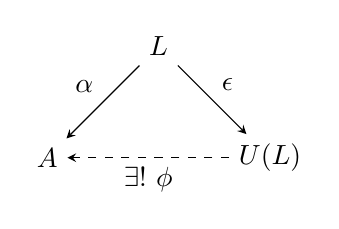
\begin{tikzpicture}[commutative diagram]
                \node (L) {$L$};
                \node (UL) [below right of=L] {$U(L)$};
                \node (A) [below left of=L] {$A$};
                \draw [arrow] (L) --(UL) node [midway, auto=left] {$\epsilon$};
                \draw [arrow] (L) --(A) node [midway, auto=right] {$\alpha$};
                \draw [arrow, dashed] (UL) --(A) node [midway, auto=below] {$\exists!\ \phi$};
            \end{tikzpicture}
        \end{center}
\end{enumerate}
\begin{insight}
    Given $(\epsilon_1, U_1)$ and $(\epsilon_2,U_2)$ we can see get maps $\phi_1: U_1\to U_2$  and $\phi_2: U_2\to U_1$ such that 
    $\phi_1\cdot\phi_2$ is identity \Todo{on $\epsilon_1(L)$} and 
    $\phi_2\cdot\phi_1$ is identity \Todo{on $\epsilon_2(L)$}. 
    But $\epsilon(L)$ generates $U(L)$, and $\phi$ is a associative algebra homomorphism, so 
    \begin{align}
        \phi\left(\sum \epsilon(x_1)\cdots\epsilon(x_n)\right) &= \sum \phi(\epsilon(x_1))\cdots\phi(\epsilon(x_n))\\
            &= \sum \epsilon(x_1)\cdots\epsilon(x_n).
    \end{align}
    Thus the compositions are identity on the whole of $U_1$ and $U_2$.
    
    %\Todo{How can we say that their composition is identity on the whole of $U_1$ and $U_2$?}
\end{insight}
Universal enveloping algebras are unique upto an isomorphism due to this universal property.

\subsection{Tensor Algebra}
\label{sub:tensor_algebra}
$i:V\to T(V)$ such that for any map $\alpha: V\to A$, where $A$ is an associative algebra, there exists an a map linear map $\psi: T(V)\to A$ such that the following diagram commutes



\begin{center}
    \begin{tikzpicture}[commutative diagram]
        \node (V) {$V$};
        \node (TV) [below right of=V] {$T(V)$};
        \node (A) [below left of=V] {$A$};
        \draw [arrow] (V) --(TV) node [midway, auto=left] {$i$};
        \draw [arrow] (V) --(A) node [midway, auto=right] {$\alpha$};
        \draw [arrow, dashed] (UL) --(A) node [midway, auto=below] {$\exists!\ \psi$};
    \end{tikzpicture}
\end{center}


\subsection{Construction}
\label{sub:construction}
Let $L$ be a Lie algebra and let $I$ be the two sided ideal generated by the elements $[x,y]-x\otimes y + y\otimes x$, then

\begin{align}
    U(L) &= T(L)/I
\end{align}

is a universal enveloping algebra for $L$.

We need to show that this satisfies the universal property. Set $V=L$ in the diagram for tensor algebra $T(V)$ to get

\begin{center}
    \begin{tikzpicture}[commutative diagram]
        \node (L) {$L$};
        \node (TL) [below right of=L] {$T(L)$};
        \node (A) [below left of=L] {$A$};
        \draw [arrow] (L) --(TL) node [midway, auto=left] {$i$};
        \draw [arrow] (L) --(A) node [midway, auto=right] {$\alpha$};
        \draw [arrow, dashed] (UL) --(A) node [midway, auto=below] {$\exists!\ \psi$};
    \end{tikzpicture}
\end{center}
If, additionally, $\alpha$ is a Lie algebra homomorphism, then 
\begin{align}
    \alpha[x,y] &= \alpha(x)\alpha(y) -\alpha(y) \alpha(x)\quad\forall x,y\in L.
\end{align}
But since $\alpha=\psi\cdot i$
\begin{align}
    \psi([x,y] -x\otimes y - y\otimes x) =0
\end{align}
Therefore $I\subset \ker \psi$, and we get that there is a unique map $\overline\phi: T/I \to A$ such that the following diagram commutes

\begin{center}
    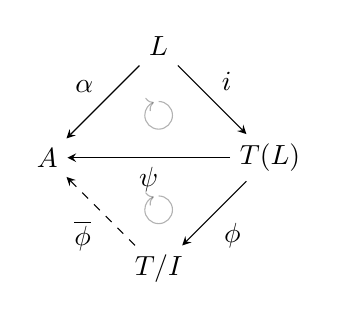
\begin{tikzpicture}[commutative diagram]
        \draw [->, opacity=0.3] (0,-0.7) arc (90:-250:5pt);
        \draw [->, opacity=0.3] (0,-1.9) arc (90:-250:5pt);

        \node (L) {$L$};
        \node (TL) [below right of=L] {$T(L)$};
        \node (A) [below left of=L] {$A$};
        \node (T/I) [below left of=TL] {$T/I$};
        \draw [arrow] (L) --(TL) node [midway, auto=left] {$i$};
        \draw [arrow] (L) --(A) node [midway, auto=right] {$\alpha$};
        \draw [arrow] (TL) --(A) node [midway, auto=below] {$\psi$};
        \draw [arrow] (TL) --(T/I) node [midway, auto=below] {$\phi$};
        \draw [arrow, dashed] (T/I) --(A) node [midway, auto=below] {$ \overline{\phi}$};
    \end{tikzpicture}
\end{center}
Thus,  we have the a lie algebra $T/I$ and a map $\epsilon=\phi\cdot i: L\to T/I$ such that the universal property is satisfied. \qed



\subsection{Extension of Lie algebra homorphism to its UEA}
\label{sub:extension_of_lie_algebra_homorphism_to_its_uea}
Given map $h: L\to M$ between two lie algebras $L$ and $M$, the universal property implies the existence of a associative algebra homomorphism $U(L)\to U(M)$ as shown in the diagram:
\begin{center}
    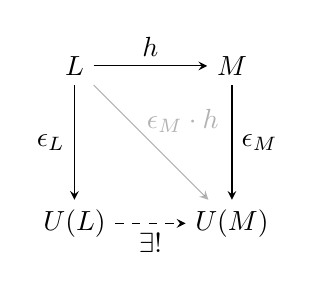
\begin{tikzpicture}[commutative diagram]
        \node (L) {$L$};
        \node (M) [right of=L] {$M$};
        \node (UL) [below of=L] {$U(L)$};
        \node (UM) [right of=UL] {$U(M)$};
        \draw [arrow] (L) -- (M) node [midway, above] {$h$};
        \draw [arrow] (L) -- (UL) node [midway, left] {$\epsilon_L$};
        \draw [arrow] (M) -- (UM) node [midway, right] {$\epsilon_M$};
        \draw [arrow, opacity=0.3] (L) -- (UM) node [midway, auto,  shift={(-5pt,0pt)}] {$\epsilon_M\cdot h$};
        \draw [arrow, dashed] (UL) -- (UM) node [midway, below] {$\exists !$};
    \end{tikzpicture}
\end{center}


\subsection{UEA of a direct sum}
\label{sub:uea_of_a_direct_sum}

\begin{align}
    U(L_1\oplus L_2) &\isomorphic U(L_1) \otimes U(L_2)
\end{align}

\subsection{Bialgebra structure}
\label{sub:bialgebra_structure}
\begin{definition}[Bialgebra]
A vector space $C$ with a map (\emph{comultiplication}) $\Delta: C\to C\otimes C$ and a map (\emph{co-unit}) $\varepsilon: D\to k$ satisfying
\begin{align}
    (\varepsilon\otimes \id) \circ \Delta &= \id \quad\text{and} \\
    (\id\otimes \varepsilon) \circ \Delta &= \id
\end{align}
is called a \emph{co-algebra}. If $C$ is an algebra and both $\Delta$ and $\varepsilon$ are algebra homomorphisms, we say that $C$ is a \emph{bi-algebra}.
    
\end{definition}

Let $L$ be any lie algebra. The map $f: L\to U(L)\otimes U(L)$ defined by
\begin{align}
    x\mapsto f(x)=x\otimes 1 + 1\otimes x
\end{align}
is a Lie algebra homomorphism. This can be seen by
\begin{align}
    f(x)f(y)- f(y)f(x) &= [x,y]\otimes 1 + 1\otimes [x,y]\\
        &= f[x,y].
    %f([x,y]) &= f(x\otimes y - y\otimes x) 
\end{align}
Thus this map induces a map $\Delta: U(L)\to U(L)\otimes U(L)$ as seen in the following commutative diagram.
\begin{center}
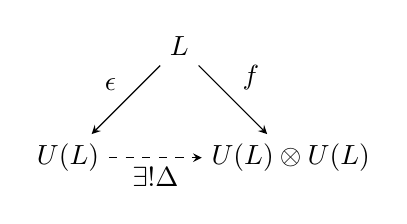
\begin{tikzpicture}[commutative diagram]
    \node (L) {$L$};
    \node (ULxUL) [below right of=L] {$U(L)\otimes U(L)$};
    \node (UL) [below left of=L] {$U(L)$};
    \draw [arrow] (L) -- (ULxUL) node [midway, auto=left] {$f$};
    \draw [arrow] (L) -- (UL) node [midway, auto=right] {$\epsilon$};
    \draw [arrow, dashed] (UL) -- (ULxUL) node [midway, below] {$\exists! \Delta$};
\end{tikzpicture}
\end{center}
Now, define the map $\varepsilon: U(L)\to k$ as
\begin{equation}
    \epsilon(x) = \begin{cases} 
        1 &\text{if } x=1,\\
        0 &\text{for all } x\in L
    \end{cases}
\end{equation}
and extend this as an algebra homorphism.
\begin{proposition}
   $(U(L), \Delta, \varepsilon)$  is a bialgebra.
\end{proposition}
\begin{proof}
    \Todo{complete this} 
\end{proof}

\subsection{The Poincar\'e-Birkhoff-Witt Theorem.}
\label{sub:the_poincar'e_birkhoff_witt_theorem_}

\Todo{Complete this section.}

\begin{theorem}[Poincar\'e-Birkhoff-Witt]
    \begin{align}
        S(L) \isomorphic \gr U(L)
    \end{align}
\end{theorem}




\chapter{Lie Algebras}
\label{cha:lie_algebras}
In this chapter, we undertake a systematic study of Lie algebras and attempt to classify them.

\section{Overview}
%\label{sec:overview}




\begin{theorem}[Ado's theorem]
Every finite dimensional lie algebra is a subalgebra of $\LieGL(V)$.
\end{theorem}

Let's make a few definitions.
\begin{align}
    D\LieG &= [\LieG, \LieG] &\text{}\\
    D_k\LieG &= [\LieG, D_{k-1}\LieG] &\text{lower central series}\\
    D^k\LieG &= [D^{k-1}\LieG, D^{k-1}\LieG] &\text{derived series}
\end{align}

\begin{definition} A lie algebra $\LieG$ is 
    \begin{enumerate}[(i)]
        \makethislistcompact
        \item \textbf{nilpotent} if $D_k\LieG=0$ for some $k$,
        \item \textbf{solvable} if $D^k\LieG=0$ for some $k$, and
        \item \textbf{semi-simple} if it has no non nonzero solvable ideals.
    \end{enumerate}
\end{definition}

\begin{definition}[Radical]
    Sum of all solvable ideals in $\LieG$ is again a solvable ideal, called the the \textbf{radical} of $\LieG$ and denoted by $\Rad(\LieG)$
\end{definition}

\begin{definition}[Reductive]
    A lie algebra $\LieG$ is \textbf{reductive} if it is the direct sum of a semisimple lie algebra and an abelian lie algebra.
\end{definition}
\begin{insight}
   It does not make much sense to classify lie algebras and keep $\Lie{gl}_n$ out of it. That's why we define reductive lie algebras. Even though $\Lie{gl}_n$ is not semi-simple, it is reductive as $\Lie{gl}_n = \Lie{sl}_n\oplus \Lie{t}$ is the direct sum of the traceless lie algebra with with the scalar lie algebra.
\end{insight}

\begin{lemma}
    $ (\mathfrak{a} + \mathfrak{b})/\mathfrak{b} \isomorphic \mathfrak a / (\mathfrak a \cap \mathfrak b) $
\end{lemma}
\begin{proof} The kernel of the composite map 
   \begin{align}
       \LieA + \LieB \onto \LieA \onto \LieA/(\LieA \cap \LieB)
   \end{align} 
   is the ideal $\LieB \in \LieA + \LieB$.
\end{proof}


Notice that the lie algebra $\LieG/\Rad(\LieG)$ is semisimple. Any lie algebra fits into the exact sequence
\begin{align}
    0\to \Rad(\LieG) \to \LieG \to \LieG/\Rad(\LieG) \to 0
\end{align}
where the first algebra is solvable and the last algebra is semisimple. Our approach to classify representations of Lie  algebras is then to study the representations of solvable and semisimple Lie algebras.

\begin{theorem}[Lie's theorem]
    
\end{theorem}

\vspace{1em}
\hrule
\vspace{1em}

Reference: FH 8.3
\begin{proposition}
    Let $G$ be a Lie group and $\LieG$ be the its Lie algebra. Let $\LieH\in \LieG$ be a subalgebra. 
    Then the subgroup of $G$ generated by $\exp(\LieH)$ is an immersed subgroup $H$ with tangent space $T_eH=\LieH$
\end{proposition}
\begin{proof}
    \Todo{complete this.} 
\end{proof}


\begin{insight}
    Let $\{(e^{\iota \alpha t}, e^{\iota\beta t})| t\in \RR\} \subseteq S^2 $. This is dense in $S^2$ if $\alpha/\beta$ is irrational. So, it's not closed. It's important to keep in mind the difference in closed and immersed groups. 
\end{insight}



\section{Covering Space}
\label{sec:covering_space}

\begin{figure}[h]
    \centering
    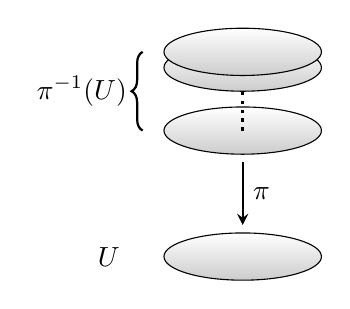
\begin{tikzpicture}[disc/.style={top color=white, bottom color=white!80!black}]
        \def\dist{0.2}
        \def\xrad{1}
        \def\yrad{0.3}
        \draw [disc] (0,-13*\dist) ellipse [start angle=0, end angle=360, x radius=\xrad, y radius=\yrad] node (U) {};
        \draw [-stealth, thick] (0,-7*\dist) -- (0,-11*\dist) node [midway, right] {$\pi$};
        \draw [disc] (0,-5*\dist) ellipse [start angle=0, end angle=360, x radius=\xrad, y radius=\yrad] node (bottom) {};
        \draw [dotted, very thick] (0,-5*\dist) -- (0,-\dist);
        \draw [disc] (0,-\dist) ellipse [start angle=0, end angle=360, x radius=\xrad, y radius=\yrad];
        \draw [disc] ellipse [start angle=0, end angle=360, x radius=\xrad, y radius=\yrad] node (top) {};

        \node [left of=U, node distance=1.7cm] {$U$};

        %\begin{scope}[shift={(-1.5cm,0cm)}]
        %\draw [decorate, decoration={brace, mirror, amplitude=2pt}] node [left of=top, node distance=1.5cm] {} -- node [left of=bottom] {};
        \def\xx{1.2cm}
        \draw [decorate, decoration={brace, mirror, amplitude=4pt, raise=2pt}, thick] ($(top)- (\xx,0)$) -- ($(bottom) - (\xx,0)$) node [midway, left, xshift=-4pt] {$\pi^{-1}(U)$};
        %\end{scope}

    \end{tikzpicture}
\end{figure}

A covering space is a space $C$ with a continuous \emph{surjective} map 
\begin{align}
    \pi: C\to X
\end{align}
such that for any point $x\in X$, there exists an open neighbourhood $U$ of $x$ such that 
\begin{align}
    \pi^{-1}(U)   &=  \coprod U_\alpha \quad\text{and}\\
    \pi|_{U_\alpha}&: U_\alpha \xrightarrow{\isomorphic} U
\end{align}
where the $U_\alpha$ are open sets and $\coprod$ is the disjoint union.
\begin{insight}
    Example 
    \begin{align}
        \RR\onto \RR/\ZZ
    \end{align}
    Every quotient is not a cover.
\end{insight}

\subsection{Universal Cover}
\label{sub:universal_cover}


A covering space is a \emph{universal covering space} if it is simply connected. 

It is universal in the sense that if there is any other cover $C$ of $X$, then there is a covering map $f: D\to C$ such that following diagram commutes
\begin{center}
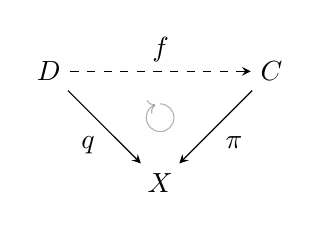
\begin{tikzpicture}[commutative diagram]
    \node [] (X) {$X$};
    \node [above left of=X] (D) {$D$};
    \node [above right of=X](C) {$C$};

    \draw [arrow] (D) -- (X) node [midway, auto=right] {$q$};
    \draw [arrow, dashed] (D) -- (C) node [midway, above] {$f$};
    \draw [arrow] (C) -- (X) node [midway, auto=left] {$\pi$};

    \draw [->, opacity=0.3] (0,1) arc (90:-250:5pt);

    
\end{tikzpicture}
\end{center}

\begin{insight}
   The universal cover of the space $X$ covers all the connected covers of the space $X$.
\end{insight}

\subsection{Second Principle}
\label{sub:second_principle}

Let $G$ and $H$ be Lie groups, $G$ is simply connected. Let $\LieG, \LieH$ be the associated Lie algebras. A linear map $\alpha: \LieG \to \LieH$ is the differential of a map $A: G\to H$ of Lie groups if and only if $\alpha$ is a map of Lie algebras.

\begin{proposition}
   A linear map $\alpha: \LieH \to \LieG$  is an isomorphism iff $A: H\to G$ is an isogeny.
\end{proposition}

\begin{proof}  {[\Todo {Sanitize; Lecture 10.17.2014}]} \\
Isogeny implies that there exists a $U\ni I_h$, such that
\begin{align}
    \varphi|_U : U_h \xrightarrow{\ \isomorphic\ } \varphi(U_h)
\end{align}
is an isomorphism.
Suppose, conversely, that $d\varphi: \LieH\to \LieG$ is an isomorphism. Then there exists a neibourhood $U\ni I_h$ such that $    \varphi: U\to \varphi(U)$ is an isomorphism.

\begin{align}
    \varphi^{-1} (I_g) &= \bigcup_\alpha h_\alpha 
\end{align}
If $h_\alpha \neq I$, then $h_\alpha \not\in U$. Therefore, $\bigcup h_\alpha$ is a disjoint union.


Then $\coprod_\alpha U h_\alpha h\to \varphi(U)g$  is the cover of $U_g$ whenever $\varphi(h)=g$.

\end{proof}

\subsection{A bit on isogeny}
\label{sub:a_bit_on_isogeny}

Let $G$ be a group, $H$ a connected manifold. Let $\varphi: H\to G$ be a covering space map. Let $e' \mapsto e_G$. Then there exists a unique Lie group structure on $H$ such that  $e' = \id_H$ and $\varphi: H\to G$ is a Lie group morphism.

\begin{proposition}
   Let   
\end{proposition}

\begin{proof}[Proof of Second Pricniple]
    \Todo{Complete this}
\end{proof}

\section{Rough Classification of Lie Algebras}
\label{sec:rough_classification_of_lie_algebras}

We have three major theorems in this section:
\begin{enumerate}
    \makethislistcompact
    \item Engel's theorem,
    \item Lie'e theorem,
    \item Levi decomposition theorem,
    \item Ado's theorem
\end{enumerate}

\subsection{Levi decomposition}
\label{sub:levi_decomposition}

We have the short exact sequence
\begin{align}
    \Rad \LieG \hookrightarrow \LieG \onto \LieG/\Rad\LieG
\end{align}
Levi's theorem basically states that this sequence splits, that is, there is an subspace $\Lie{l}$ such that
\begin{align}
    \LieG = \Lie{l}\oplus\Rad\LieG
\end{align}

\hrule\vspace{1em}
\Todo{Sanitize; Lecture 10.17.2014}

\begin{theorem}
   Let $\LieG$  be a lie algebra with the radical $\Lie r$. There exists a subalgebra $\Lie l$ such that $\Lie g = \Lie l \oplus \Lie r$.
\end{theorem}
\begin{insight}
    This looks very much like 
    \begin{align}
        \begin{pmatrix}  x& y \\ 0 & z \end{pmatrix} &= \begin{pmatrix} x & 0 \\ 0 & z \end{pmatrix} + \begin{pmatrix} 0 & y \\ 0 & 0  \end{pmatrix}
    \end{align} 
\end{insight}
\begin{proof}
    Reduction step: No non-zero ideal is properly contained in $\Lie r$. (Otherwise if $\Lie i\subset \Lie r, $) \Todo{....Complete this}
\end{proof}

\subsection{Engel's theorem}
\label{sub:engel_s_theorem}

\begin{theorem}[Engel]
    
\end{theorem}





















%%%%%%%%%%%%%%%%%%%%%%%%%%%%%%%%%%%%%%%%%%%%%%%%%%%%%%%%%%%%%%%%%%%%%%%%%
% APPENDICES
%%%%%%%%%%%%%%%%%%%%%%%%%%%%%%%%%%%%%%%%%%%%%%%%%%%%%%%%%%%%%%%%%%%%%%%%%
\appendix
\chapter{Tensor Product}
\label{cha:tensor_product}

Let $V,\ W$ be vector spaces. A tensor product is a vector space $V\otimes W$ equipped with a bilinear map
\begin{align}
    V\times W \to V\otimes W\\
    (v,w) \mapsto v\otimes w
\end{align}
such that it is \emph{universal}. That is, given any other vector space $U$ and a bilinear map $\beta: V\times W\to U$, there is unique map $\beta': V\otimes W \to U$ such that $\beta'(v\otimes w) = \beta(v,w)$. The following diagram commutes:

\begin{center}
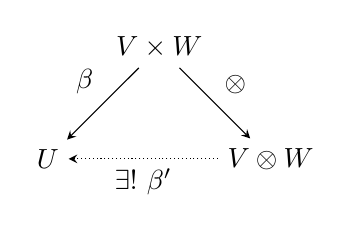
\begin{tikzpicture}[commutative diagram] 
    \node (a) {$V\times W$};
    \node (b) [below right of=a] {$V\otimes W$};
    \node (c) [below left of=a] {$U$};
    \draw [arrow] (a) -- (b) node [midway] {$\otimes$};
    \draw [arrow] (a) -- (c) node [midway,auto=right] {$\beta$};
    \draw [exists] (b) -- (c) node [midway] {$\exists!\ \beta'$};
\end{tikzpicture}
\end{center}
The universality requirement means that the tensor product thus defined is unique upto an isomorphism. Let there be another tensor product $V\otimes' W$ (a vector space and a correspoding map that takes $(v,w)\mapsto v\otimes' w$) that is also universal. Then it immediately implies that there is a bijection between $V\otimes W$ and $V\otimes' W$ since
\begin{center}
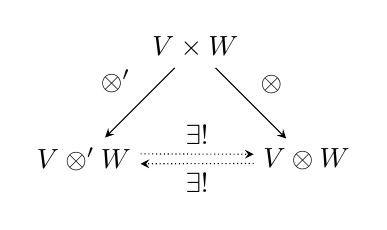
\begin{tikzpicture}[commutative diagram] 
    \node (a) {$V\times W$};
    \node (b) [below right of=a] {$V\otimes W$};
    \node (c) [below left of=a] {$V\otimes' W$};
    \draw [arrow] (a) -- (b) node [midway] {$\otimes$};
    \draw [arrow] (a) -- (c) node [midway,auto=right] {$\otimes'$};
    \draw [exists] (c.5) -- (b.175) node [midway, above] {$\exists!$};
    \draw [exists] (b.185) -- (c.355) node [midway] {$\exists!$};
\end{tikzpicture}
\end{center}

\begin{theorem}[]
    $\Hom(V,W) \isomorphic V^*\otimes W$ as vector spaces.
\end{theorem}
\begin{proof}
   Quick Check: Set $W=\CC$ so that we get $\Hom(V,\CC)\isomorphic V^*\otimes 1 = V^*$, which is the definition of the dual space $V^*$.

   Given $(\beta: V\to W) \in \Hom(V,W)$, define the map $\phi: \Hom(V,W)\to V^* \otimes W $ such that 
   \begin{align}
       \phi(\beta) = \sum_{i,j} \beta_{ij} v_i^* \otimes w_j
   \end{align}
   where $\{v_i\}$ and $\{w_j\}$ are orthonormal basis for $V$ and $W$ respectively and $\beta_{ij} = \beta(v_i)^T w_j$.
   This is a homorphism of vector spaces. The inverse map is obvious.
\end{proof}

\section{Exterior Products and Symmetric Products}
\label{sec:exterior_products_and_symmetric_products}

\subsection{Definitions}
\label{sub:definitions}

\subsection{Some Combinatorics}
\label{sub:some_combinatorics}

Lets find out the dimensions of the vector space $\Lambda^k V$, where $V$ is an $n$-dimensional vector space.
If $\{e_i\}$ is a basis for $V$, we know that a basis for $\Lambda^k V$ is 
\begin{align}
    \{e_{i_1}\wedge e_{i_2} \wedge\cdots \wedge e_{i_k} : i_1 < i_2 < \cdots < i_k \}.
\end{align}
How many vectors are there in this basis? This can be asnwered by looking at how many ways are there to simply choose $k$ objects from a set of $n$ different objects. Since there is just one of arranging them (in increasing order), that would be the number of vectors in the basis. So,
\begin{align}
    \dim \Lambda^k (V) &= {}^{\dim V}C_k
    \label{eqn:dim_exteriorpower}
\end{align}

What's the dimension of $\Sym^k(V)$? The basis is
\begin{align}
    \{e_{i_1}\cdot e_{i_2} \cdot\cdots \cdot e_{i_k} : i_1 \leq i_2 \leq \cdots \leq i_k \}.
\end{align}
Another way to write that is
\begin{align}
    \{e_1^{a_1}\cdot e_2^{a_2} \cdots e_k^{a_k}\},\quad\text{such that } \sum_i a_i = n,\, a_i\geq 0.
\end{align}
We just need to know how many ways are there to distribute $n$ identical things among $k$ different people with no restriction on the number of things anyone can get. To solve this, introduce $k-1$ identical barriers (denoted by $|$) between $n$ things (denoted by $\circ$)and look at the number of permutations.
\begin{align}
    \circ | \circ | \cdots | \circ
\end{align}
Every permutation here gives possible choice of ${a_1,\dotsc,a_k}$. Therefore,
\begin{align}
    \dim (\Sym^k (V)) &= {}^{\dim V +k-1}C_{k}
    \label{eqn:dim_symmetricpower}
\end{align}


\chapter{General Information}

\section{Resources}
\label{sec:Resources}
Here are some resources that I found useful while preparing these notes
\begin{itemize}
    \item Representation Theory - A First Course by \emph{Fulton, Harris}
\end{itemize}


%%%%%%%%%%%%%%%%%%
%  Bibliography  %
%%%%%%%%%%%%%%%%%%
\nocite{*} % Print all entries in the bib file
\printbibliography

\end{document}
